%%%%%%%%%%%%%%%%%%%%%%%%%%%%%%%%%%%%%%%%%%%%%%%%%%%%%%%%%%%%%%%
%% BRIEF VERSION OF OXFORD THESIS TEMPLATE FOR CHAPTER PREVIEWS

%%%%% CHOOSE PAGE LAYOUT
% format for PDF output (ie equal margins, no extra blank pages):
\documentclass[a4paper,nobind]{templates/ociamthesis}

% UL 5 January 2021 - add packages used by kableExtra
\usepackage{booktabs}
\usepackage{longtable}
\usepackage{array}
\usepackage{multirow}
\usepackage{wrapfig}
\usepackage{colortbl}
\usepackage{pdflscape}
\usepackage{tabu}
\usepackage{threeparttable}
\usepackage{threeparttablex}
\usepackage[normalem]{ulem}
\usepackage{makecell}
\usepackage[colorlinks=false,pdfpagelabels,hidelinks=]{hyperref}
\usepackage{float}


%UL set section header spacing
\usepackage{titlesec}
% 
\titlespacing\subsubsection{0pt}{24pt plus 4pt minus 2pt}{0pt plus 2pt minus 2pt}

% UL 30 Nov 2018 pandoc puts lists in 'tightlist' command when no space between bullet points in Rmd file
\providecommand{\tightlist}{%
  \setlength{\itemsep}{0pt}\setlength{\parskip}{0pt}}
 
% UL 1 Dec 2018, fix to include code in shaded environments
\usepackage{color}
\usepackage{fancyvrb}
\newcommand{\VerbBar}{|}
\newcommand{\VERB}{\Verb[commandchars=\\\{\}]}
\DefineVerbatimEnvironment{Highlighting}{Verbatim}{commandchars=\\\{\}}
% Add ',fontsize=\small' for more characters per line
\usepackage{framed}
\definecolor{shadecolor}{RGB}{248,248,248}
\newenvironment{Shaded}{\begin{snugshade}}{\end{snugshade}}
\newcommand{\AlertTok}[1]{\textcolor[rgb]{0.94,0.16,0.16}{#1}}
\newcommand{\AnnotationTok}[1]{\textcolor[rgb]{0.56,0.35,0.01}{\textbf{\textit{#1}}}}
\newcommand{\AttributeTok}[1]{\textcolor[rgb]{0.77,0.63,0.00}{#1}}
\newcommand{\BaseNTok}[1]{\textcolor[rgb]{0.00,0.00,0.81}{#1}}
\newcommand{\BuiltInTok}[1]{#1}
\newcommand{\CharTok}[1]{\textcolor[rgb]{0.31,0.60,0.02}{#1}}
\newcommand{\CommentTok}[1]{\textcolor[rgb]{0.56,0.35,0.01}{\textit{#1}}}
\newcommand{\CommentVarTok}[1]{\textcolor[rgb]{0.56,0.35,0.01}{\textbf{\textit{#1}}}}
\newcommand{\ConstantTok}[1]{\textcolor[rgb]{0.00,0.00,0.00}{#1}}
\newcommand{\ControlFlowTok}[1]{\textcolor[rgb]{0.13,0.29,0.53}{\textbf{#1}}}
\newcommand{\DataTypeTok}[1]{\textcolor[rgb]{0.13,0.29,0.53}{#1}}
\newcommand{\DecValTok}[1]{\textcolor[rgb]{0.00,0.00,0.81}{#1}}
\newcommand{\DocumentationTok}[1]{\textcolor[rgb]{0.56,0.35,0.01}{\textbf{\textit{#1}}}}
\newcommand{\ErrorTok}[1]{\textcolor[rgb]{0.64,0.00,0.00}{\textbf{#1}}}
\newcommand{\ExtensionTok}[1]{#1}
\newcommand{\FloatTok}[1]{\textcolor[rgb]{0.00,0.00,0.81}{#1}}
\newcommand{\FunctionTok}[1]{\textcolor[rgb]{0.00,0.00,0.00}{#1}}
\newcommand{\ImportTok}[1]{#1}
\newcommand{\InformationTok}[1]{\textcolor[rgb]{0.56,0.35,0.01}{\textbf{\textit{#1}}}}
\newcommand{\KeywordTok}[1]{\textcolor[rgb]{0.13,0.29,0.53}{\textbf{#1}}}
\newcommand{\NormalTok}[1]{#1}
\newcommand{\OperatorTok}[1]{\textcolor[rgb]{0.81,0.36,0.00}{\textbf{#1}}}
\newcommand{\OtherTok}[1]{\textcolor[rgb]{0.56,0.35,0.01}{#1}}
\newcommand{\PreprocessorTok}[1]{\textcolor[rgb]{0.56,0.35,0.01}{\textit{#1}}}
\newcommand{\RegionMarkerTok}[1]{#1}
\newcommand{\SpecialCharTok}[1]{\textcolor[rgb]{0.00,0.00,0.00}{#1}}
\newcommand{\SpecialStringTok}[1]{\textcolor[rgb]{0.31,0.60,0.02}{#1}}
\newcommand{\StringTok}[1]{\textcolor[rgb]{0.31,0.60,0.02}{#1}}
\newcommand{\VariableTok}[1]{\textcolor[rgb]{0.00,0.00,0.00}{#1}}
\newcommand{\VerbatimStringTok}[1]{\textcolor[rgb]{0.31,0.60,0.02}{#1}}
\newcommand{\WarningTok}[1]{\textcolor[rgb]{0.56,0.35,0.01}{\textbf{\textit{#1}}}}

%UL 2 Dec 2018 add a bit of white space before and after code blocks
\renewenvironment{Shaded}
{
  \vspace{10pt}%
  \begin{snugshade}%
}{%
  \end{snugshade}%
  \vspace{8pt}%
}
%UL 2 Dec 2018 reduce whitespace around verbatim environments
\usepackage{etoolbox}
\makeatletter
\preto{\@verbatim}{\topsep=0pt \partopsep=0pt }
\makeatother

%UL 28 Mar 2019, enable strikethrough
\usepackage[normalem]{ulem}

%UL use soul package for correction highlighting
\usepackage{soul}
\usepackage{xcolor}
\newcommand{\ctext}[3][RGB]{%
  \begingroup
  \definecolor{hlcolor}{#1}{#2}\sethlcolor{hlcolor}%
  \hl{#3}%
  \endgroup
}
\soulregister\ref7
\soulregister\cite7
\soulregister\autocite7
\soulregister\textcite7
\soulregister\pageref7

%UL 3 Nov 2019, avoid mysterious error from not having hyperref included
\usepackage{hyperref}

%%%%% SELECT YOUR DRAFT OPTIONS
% Three options going on here; use in any combination.  But remember to turn the first two off before
% generating a PDF to send to the printer!

% This adds a "DRAFT" footer to every normal page.  (The first page of each chapter is not a "normal" page.)

% This highlights (in blue) corrections marked with (for words) \mccorrect{blah} or (for whole
% paragraphs) \begin{mccorrection} . . . \end{mccorrection}.  This can be useful for sending a PDF of
% your corrected thesis to your examiners for review.  Turn it off, and the blue disappears.

%%%%% BIBLIOGRAPHY SETUP
% Note that your bibliography will require some tweaking depending on your department, preferred format, etc.
% The options included below are just very basic "sciencey" and "humanitiesey" options to get started.
% If you've not used LaTeX before, I recommend reading a little about biblatex/biber and getting started with it.
% If you're already a LaTeX pro and are used to natbib or something, modify as necessary.
% Either way, you'll have to choose and configure an appropriate bibliography format...

% The science-type option: numerical in-text citation with references in order of appearance.
% \usepackage[style=numeric-comp, sorting=none, backend=biber, doi=false, isbn=false]{biblatex}
% \newcommand*{\bibtitle}{References}

% The humanities-type option: author-year in-text citation with an alphabetical works cited.
% \usepackage[style=authoryear, sorting=nyt, backend=biber, maxcitenames=2, useprefix, doi=false, isbn=false]{biblatex}
% \newcommand*{\bibtitle}{Works Cited}

%UL 3 Dec 2018: set this from YAML in index.Rmd
\usepackage[style=numeric-comp, sorting=none, backend=biber, doi=false, isbn=false]{biblatex}
\newcommand*{\bibtitle}{References}

% This makes the bibliography left-aligned (not 'justified') and slightly smaller font.
\renewcommand*{\bibfont}{\raggedright\small}

% Change this to the name of your .bib file (usually exported from a citation manager like Zotero or EndNote).
\addbibresource{references.bib}

%%%%% YOUR OWN PERSONAL MACROS
% This is a good place to dump your own LaTeX macros as they come up.

\newcommand{\Sc}{\mathcal{S}}
\newcommand{\R}{\mathcal{R}}
\newcommand{\N}{\mathcal{N}}
\newcommand{\X}{\mathcal{X}} 
\newcommand{\m}{\mathbf{m}}
\newcommand{\bu}{\mathbf{u}}
\newcommand{\bv}{\mathbf{v}}
\newcommand{\w}{\mathbf{w}}
\newcommand{\x}{\mathbf{x}}
\newcommand{\y}{\mathbf{y}}
\newcommand{\z}{\mathbf{z}}
\newcommand{\bb}{\mathbf{b}}
\newcommand{\bphi}{\bm{\phi}}
\newcommand{\brho}{\bm{\rho}}
\newcommand{\btheta}{\bm{\theta}}

\RequirePackage{bm}

% To make text superscripts shortcuts
	\renewcommand{\th}{\textsuperscript{th}} % ex: I won 4\th place
	\newcommand{\nd}{\textsuperscript{nd}}
	\renewcommand{\st}{\textsuperscript{st}}
	\newcommand{\rd}{\textsuperscript{rd}}

%%%%% THE ACTUAL DOCUMENT STARTS HERE
\begin{document}

%%%%% CHOOSE YOUR LINE SPACING HERE
% This is the official option.  Use it for your submission copy and library copy:
\setlength{\textbaselineskip}{22pt plus2pt}
% This is closer spacing (about 1.5-spaced) that you might prefer for your personal copies:
%\setlength{\textbaselineskip}{18pt plus2pt minus1pt}

% UL: You can set the general paragraph spacing here - I've set it to 2pt (was 0) so
% it's less claustrophobic
\setlength{\parskip}{2pt plus 1pt}

% Leave this line alone; it gets things started for the real document.
\setlength{\baselineskip}{\textbaselineskip}

% all your chapters and appendices will appear here
\hypertarget{bayes-st}{%
\chapter{Bayesian spatio-temporal statistics}\label{bayes-st}}

\adjustmtc
\markboth{Bayesian}{}

\hypertarget{bayesian-statistics}{%
\section{Bayesian statistics}\label{bayesian-statistics}}

Bayesian statistics is a mathematical paradigm for learning from data.
I provide a brief, opinionated, overview in this section, and recommend \textcite{mcelreath2020statistical} or \textcite{gelman2013bayesian} for a more complete introduction.

\hypertarget{bayesian-modelling}{%
\subsection{Bayesian modelling}\label{bayesian-modelling}}

At its best, the Bayesian paradigm allows the analyst focus their attention on the question of how to model the data.
This is achieved by the construction of a generative model \(p(\y, \bvartheta)\) for the observed data \(\y\) together with parameters \(\bvartheta\).
The model is generative in the sense that one can simulate from it to obtain draws \((\y, \bvartheta) \sim p(\y, \bvartheta)\) in what is known as a prior predictive check.
If these draws differ too greatly from what the analyst would expect, then the generative model can be refined.

The model is usually constructed from two parts, known as the likelihood \(p(\y \, | \, \bvartheta)\) and the prior \(p(\bvartheta)\) whereby \(p(\y, \bvartheta) = p(\y \, | \, \bvartheta) p(\bvartheta)\).
The likelihood, as a function of \(\bvartheta\) with \(\y\) fixed, reflects the probability of observing the data when the true value of the parameters is \(\bvartheta\).
The prior encapsulates beliefs about the parameters \(\bvartheta\) before the data is observed.
There are substantial disagreements about how the prior should be specified.
That said, the distinction between likelihood and prior can sometimes be blurred (Section \ref{hierarchical-lgm-elgm}).
As such, these difficulties are not unique to the prior \autocite{gelman2017prior}.

\hypertarget{bayesian-computation}{%
\subsection{Bayesian computation}\label{bayesian-computation}}

The posterior distribution \(p(\bvartheta \, | \, \y)\) represents beliefs about the parameters given the observed data.
Using Bayes' theorem, it is given by
\begin{equation}
p(\bvartheta \, | \, \y) = \frac{p(\y \, | \, \bvartheta) p(\bvartheta)}{p(\y)}. \label{eq:posterior}
\end{equation}
Unfortunately, it is usually intractable to calculate directly because of the integral \(p(\y) = \int p(\y, \bvartheta) \text{d}\bvartheta\) in the denominator.
As such, we are typically in the situation where, athough the numerator is proportional to the posterior \(p(\bvartheta \, | \, \y) \propto p(\y \, | \, \bvartheta) p(\bvartheta)\) and easy to evaluate, it is not easy to evaluate the posterior itself.

A great variety of computational methods have been developed at to tackle this problem.
Markov chain Monte Carlo (MCMC) is the most popular approach, and proceeds by simulating samples from a Markov chain with the posterior as its stationary distribution.
Variational Bayes approaches assume the posterior distribution belongs to a certain class of functions and use optimisation to choose the best member of that class.

\hypertarget{interplay-between-modelling-and-computation}{%
\subsection{Interplay between modelling and computation}\label{interplay-between-modelling-and-computation}}

Bayesian computation aspires to abstract away calculation of the posterior distribution from the analyst.
Modern computational techniques and software have made this aspiration a reality for many models.
However, computation of the posterior remains intractable for a substantial majority of models.
As such, the analyst need not only to be concerned with choosing a model suitable for the data, but also choosing a model for which the posterior is tractable in reasonable time.
It is in this sense, that there is an interplay between modelling and computation.
As computation improves, the space of models available to the analyst expands.

\hypertarget{spatio-temporal-statistics}{%
\section{Spatio-temporal statistics}\label{spatio-temporal-statistics}}

In spatio-temporal statistics \autocite{cressie2015statistics} we observe data indexed by spatial or temporal location.
In this thesis we assume that the spatial study region \(\mathcal{S} \subseteq \mathbb{R}^2\) has two dimensions, corresponding to latitude and longitude.
Data may be associated to a point \(s \in \mathcal{S}\) or area \(A \subseteq \mathcal{S}\) in the study region.
The temporal study period \(\mathcal{T} \subseteq \mathbb{R}\) can more generally be assumed to be one dimensional.

Commonly used independent and identically distributed (IID) assumptions on observations are rarely suitable in this setting because we expect there to be spatio-temporal correlation structure.

\hypertarget{hierarchical-lgm-elgm}{%
\section{Model classes}\label{hierarchical-lgm-elgm}}

\hypertarget{hierarchical}{%
\subsection{Hierarchical models}\label{hierarchical}}

Often the data we model has hierarchical structure.
For example, we might make multiple measurements of the same unit.

\begin{figure}

{\centering 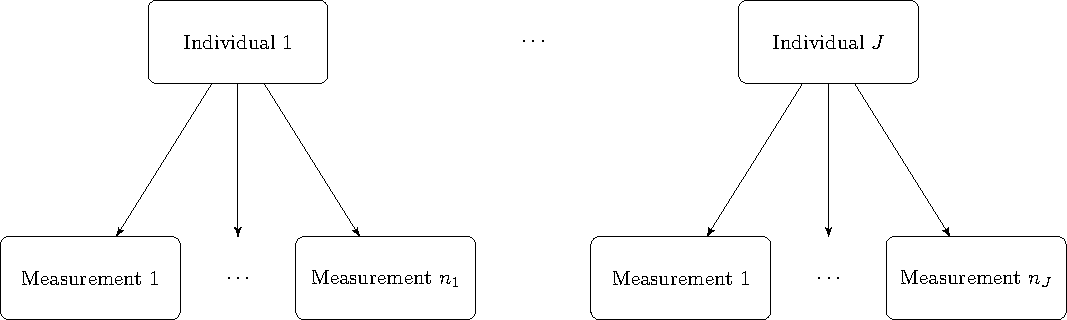
\includegraphics[width=0.95\linewidth]{figures/hierarchical-structure} 

}

\caption{Data often has a hierarchical structure.}\label{fig:chapter-flowchart}
\end{figure}

Bayesian hierarchical models are comprised of multiple stages
\begin{align*}
p(\x, \btheta \, | \, \y) \propto p(\y, \x, \btheta) = p(\y \, | \, \x, \btheta) p(\x \, | \, \btheta) p(\btheta).
\end{align*}

\hypertarget{latent-gaussian-models}{%
\subsection{Latent Gaussian models}\label{latent-gaussian-models}}

Latent Gaussian models {[}LGMs; \textcite{rue2009approximate}{]} are a class of three-stage Bayesian hierarchical models in which, loosely speaking, the middle layer is Gaussian.
More specifically, in an LGM, the likelihood is given by
\begin{align*}
y_i &\sim p(y_i \, | \, \eta_i, \theta_1), \quad i \in [n]\\
\mu_i &= \mathbb{E}(y_i \, | \, \eta_i) = g(\eta_i), \\
\eta_i &= \beta_0 + \sum_{l = 1}^{p} \beta_j z_{ji} + \sum_{k = 1}^{r} f_k(u_{ki}),
\end{align*}
where \([n] = \{1, \ldots, n\}\).
The response variable is \(\y = (y)_{i \in [n]}\) with likelihood \(p(\y \, | \, \bmeta, \btheta_1) = \prod_{i = 1}^n p(y_i \, | \, \eta_i, \btheta_1)\), where \(\bmeta = (\eta)_{i \in [n]}\).
Each response has conditional mean \(\mu_i\) with inverse link function \(g: \mathbb{R} \to \mathbb{R}\) such that \(\mu_i = g(\eta_i)\).
The vector \(\btheta_1 \in \mathbb{R}^{s_1}\), with \(s_1\) assumed small, are additional parameters of the likelihood.
The structured additive predictor \(\eta_i\) may include an intercept \(\beta_0\), linear effects \(\beta_j\) of the covariates \(z_{ji}\), and unknown functions \(f_k(\cdot)\) of the covariates \(u_{ki}\).
The parameters \(\beta_0\), \(\{\beta_j\}\), \(\{f_k(\cdot)\}\) are each assigned Gaussian priors, and can be collected into a vector \(\x \in \mathbb{R}^N\) such that \(\x \sim \mathcal{N}(\mathbf{0}, \mathbf{Q}(\btheta_2)^{-1})\) where \(\btheta_2 \in \mathbb{R}^{s_2}\) are further parameters, again with \(s_2\) assumed small.
Let \(\btheta = (\btheta_1, \btheta_2) \in \mathbb{R}^m\) with \(m = s_1 + s_2\) be all hyperparameters, with prior \(p(\theta)\).
In total, the parameters of the LGM \(\bvartheta = (\x, \btheta)\) comprise both the latent field and hyperparameters.

Spatio-temporal data are well suited to being modelled with LGMs.

\hypertarget{extended-latent-gaussian-models}{%
\subsection{Extended latent Gaussian models}\label{extended-latent-gaussian-models}}

Many of leading-edge disease mapping models fall outside the LGM class.
However, many of these models do fit into the class of extended latent Gaussian models {[}ELGMs; \textcite{stringer2021fast}{]}.
By allowing many-to-one link functions, ELGMs facilitate modelling of non-linearities.
The structured additive predictor is redefined as \(\bmeta = (\eta)_{i \in [N_n]}\), where \(N_n \in \mathbb{N}\) is a function of \(n\), and it is possible that \(N_n \neq n\).
Each mean response \(\mu_i\) now depends on some subset \(\mathcal{J}_i \subseteq [N_n]\) of indices of \(\bmeta\), with \(\cup_{i = 1}^n \mathcal{J}_i = [N_n]\) and \(1 \leq |\mathcal{J}_i| \leq N_n\).
The inverse link function \(g(\cdot)\) is redefined for each observation to be a possibly many-to-one mapping \(g_i: \mathbb{R}^{|\mathcal{J}_i|} \to \mathbb{R}\), such that \(\mu_i = g_i(\bmeta_{\mathcal{J}_i})\).
Put together, ELGMs are then of the form
\begin{align*}
y_i &\sim p(y_i \, | \, \bmeta_{\mathcal{J}_i}, \btheta_1), \quad i \in [n] \\
\mu_i &= \mathbb{E}(y_i \, | \, \bmeta_{\mathcal{J}_i}) = g_i(\bmeta_{\mathcal{J}_i}), \\
\eta_j &= \beta_0 + \sum_{l = 1}^{p} \beta_j z_{ji} + \sum_{k = 1}^{r} f_k(u_{ki}), \quad j \in [N_n],
\end{align*}
with latent field and hyperparameter priors as in the LGM case.


%%%%% REFERENCES

% JEM: Quote for the top of references (just like a chapter quote if you're using them).  Comment to skip.
% \begin{savequote}[8cm]
% The first kind of intellectual and artistic personality belongs to the hedgehogs, the second to the foxes \dots
%   \qauthor{--- Sir Isaiah Berlin \cite{berlin_hedgehog_2013}}
% \end{savequote}

\setlength{\baselineskip}{0pt} % JEM: Single-space References

{\renewcommand*\MakeUppercase[1]{#1}%
\printbibliography[heading=bibintoc,title={\bibtitle}]}

\end{document}
